% !TEX encoding = UTF-8 Unicode
% !TEX spellcheck = en_US
% !TEX root = ../../../ICMA2020.tex

\subsection{Experimental Model Application}


After the parameter identification the process-based models are tested in a classical model-based feedforward control scheme to ensure that the identified process-models are suitable for practical use. The utilized control scheme of the robot is given by Fig.\,\ref{fig:controler}. The individual joints are controlled using an independent joint control loop. 
Here $\boldsymbol{q}_\text{d}$, $\dot{\boldsymbol{q}}_\text{d}$ and $\ddot{\boldsymbol{q}}_\text{d}$ represent the desired trajectory and $\hat{\boldsymbol{\tau}}$ is the model prediction.


\begin{figure}[tb]
  \vspace{-0.2cm}
  \centering
   \input{Chapters/Experimental_Results/Experimental_Validation/Controller.pdf_tex}
   \vspace{-0.2 cm}
  \caption{Control loop of the robot.}
  \label{fig:controler}
  \vspace{-0.1cm}
\end{figure}


The process-based models are used for their respective process and are then compared to the models A and B. %The model output is added to the joint torque reference with a multiplier $k_m$. During the experiments the best results were achieved with $k_M = 0.8$.
To quantify the controller performance the root mean square value (RMS) of the reference error is calculated over all measurement points for each joint. For process 1 the RMS values of the reference errors for the different models are given in Tab.\,\ref{tab:RefErrorProcess1}.% As an example Fig. \ref{fig:ExpValProcess1} shows the reference error for process 1 in joint 4.

\begin{table}[tb]
	\caption{RMS values of the reference error for process 1 in all joints.}\label{tab:RefErrorProcess1}
	\centering
	\begin{tabular}[h]{|r|c|c|c|c|}\hline
		% !TEX encoding = UTF-8 Unicode
% !TEX spellcheck = en_US
joint	 & no Model	  & Model A	 & Model B	& Process Model	 \\ \hline 
$j$	 & $q_{e,\text{RMS},j}$ ($^{\circ}$)	  & $q_{e,\text{RMS},j}$ ($^{\circ}$)	 & $q_{e,\text{RMS},j}$ ($^{\circ}$)	 & $q_{e,\text{RMS},j}$ ($^{\circ}$)	 \\ \hline 
1	& 0.0039	& 0.0021	& 0.0022	& 0.0023	 \\ %\hline 
2	& 0.0041	& 0.0022	& 0.0022	& 0.0024	 \\ %\hline 
3	& 0.0070	& 0.0050	& 0.0049	& 0.0053	 \\ %\hline 
4	& 0.0200	& 0.0128	& 0.0127	& 0.0135	 \\ %\hline 
5	& 0.0099	& 0.0049	& 0.0048	& 0.0049	 \\ %\hline 
6	& 0.0162	& 0.0103	& 0.0096	& 0.0093	 \\ \hline 

	\end{tabular}
\end{table}

%\begin{figure}[tb]
%  \vspace{-0.2cm}
%  \centering
%   \includegraphics[width = 7.5cm]{Chapters/Experimental_Results/Experimental_Validation/Regelfehler_ProzessModell_Achse-4.pdf}
%  \caption{Reference error for process 1 in joint 4 with and without model.}
%  \label{fig:ExpValProcess1}
%  \vspace{-0.1cm}
%\end{figure}

%For process 2 the RMS values of the reference error for the different models are given in Tab. \ref{tab:RefErrorProcess2}. 
The application of all models for process 2 yields similar RMS values to process 1 and are omitted here. Fig.\,\ref{fig:ExpValProcess2} shows the trajectory of the robot end-effector in Cartesian space focused on one of the corners of the square. It can be seen, that the end-effector performs an overshoot which is typical for such a rectangular trajectory. The utilization of the model approximately halves the size of the overshoot. Fig.\,\ref{fig:ExpValProcess2} only shows the process model as a representative example, since all models yield a similar performance.

%\begin{table}[tb]
%	\caption{RMS values of the reference error for process 2 in all joints.}\label{tab:RefErrorProcess2}
%	\centering
%	\begin{tabular}[h]{|r|c|c|c|c|}\hline
%		joint	 & no Model A	  & Model A	 & Model B	& Process Model	 \\ \hline 
$j$	 & $q_{e,RMS,j}$ ($^{\circ}$)	  & $q_{e,RMS,j}$ ($^{\circ}$)	 & $q_{e,RMS,j}$ ($^{\circ}$)	 & $q_{e,RMS,j}$ ($^{\circ}$)	 \\ \hline 
1	& 0.0029	& 0.0012	& 0.0012	& 0.0012	 \\ %\hline 
2	& 0.0068	& 0.0027	& 0.0029	& 0.0031	 \\ %\hline 
3	& 0.0115	& 0.0106	& 0.0103	& 0.0101	 \\ %\hline 
4	& 0.0001	& 0.0002	& 0.0003	& 0.0001	 \\ %\hline 
5	& 0.0090	& 0.0056	& 0.0050	& 0.0044	 \\ %\hline 
6	& 0.0244	& 0.0098	& 0.0112	& 0.0255	 \\ \hline 

%	\end{tabular}
%\end{table}

\begin{figure}[tb]
  \vspace{-0.2cm}
  \centering
   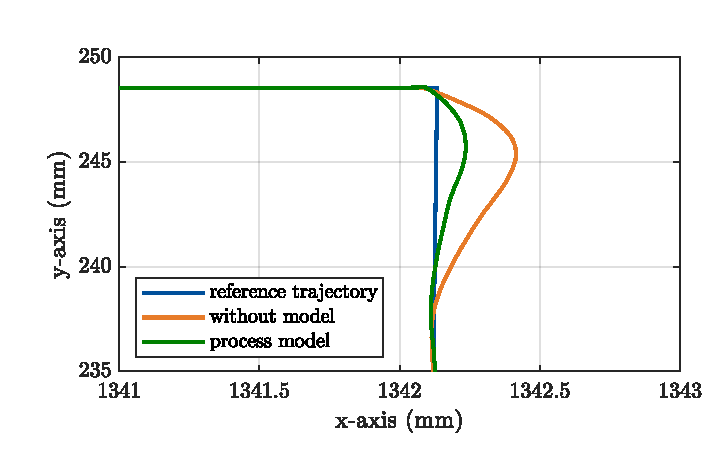
\includegraphics[width = 7.5cm]{Chapters/Experimental_Results/Experimental_Validation/EE_square.pdf}
   \vspace{-0.5cm}
  \caption{Reference and actual trajectory of the end-effector in Cartesian space.}
  \label{fig:ExpValProcess2}
  \vspace{-0.1cm}
\end{figure}

In general both process-based models perform similar to the models A and B which were derived from a classical parameter identification. This shows that the process based-models are suitable for practical application.% On average the model based feed-forward control scheme, utilizing the process models, reduces the control error by a factor of 3. This shows that the process based models are suitable for practical application.